\section{Effective One-Particle Theories}
The most widely used ground-state QMC method, FN-DMC, requires a trial wave function $\Psi_T$ to start the imaginary time projection process.
The node of $\Psi_T$ directly controls the one uncontrolled error, the fixed-node error, in the DMC total energy.
Even bosonic details of $\Psi_T$ can matter to observables that do not commute with the hamiltonian due to the mixed-estimator error.
Further, the complexity of $\Psi_T$ affects the efficiency of a DMC run, because $\Psi_T$ and many its derivatives need to be evaluated at every step of the algorithm.
Therefore, accurate and compact trial wave functions are crucial for practical high-accuracy DMC simulations.

While it is possible to construct such trial wave functions analytically~\cite{Holzmann2003,Holzmann2006,Pierleoni2008}, the process is rather involved and requires deep understanding of the particular system being simulated.
For a generic material, it is much easier to base the many-body trial wave function on existing mean-field theory or effective one-electron theory that approximately include some effects of electron correlation.
%to construct a non-interacting trial wave function  to construct a trial wave function
This chapter introduces one theory in each of these two categories.

\subsection{Hartree-Fock}

\subsubsection{The Hartree-Fock Equations}
The Hartree-Fock (HF) equations are a set of equations that couple spin orbitals in a determinant wave function. They can be obtained by minimizing the energy of a Slater determinant with the constraint that spin orbitals remain orthonormal. If each molecular orbital $a$ is written as a linear combination of a set of basis functions $\{\phi_\mu\}$
\begin{align} \label{eq:hf-psia}
\psi_a = \sum\limits_{\mu=1}^K C_{\mu a} \phi_\mu,
\end{align}
then the constraint optimization problem can be converted to a set of linear equations, resulting in an eigenvalue problem.
However, the eigenvectors of this linear problem are needed to construct the problem to be solved.
This self-consistency requirement makes the HF equations non-linear, thus requiring an iterative solver.
Once an initial guess for the eigenvectors $C_{\mu a}$ have been chosen, one can construct the linear problem to be solved via a \emph{Fock matrix}.
For a spin-unpolarized system $N_{\up}=N_{\dn}=N/2$, the restricted Hartree-Fock (RHF) solution is defined by the first $N/2$ eigenvectors of the Fock matrix
\begin{align}
F_{\mu\nu} = \hcore + \sum\limits_{\lambda\sigma} P_{\lambda\sigma} \left[
(\mu\nu|\sigma\lambda) - \frac{1}{2}(\mu\lambda|\sigma\nu)
\right],
\end{align} % (3.154)
where $P_{\lambda\sigma}=2\sum_{a=1}^{N/2} C_{\lambda a}C_{\sigma a}^*$ is the density matrix of the trial states. The \textit{Coulomb integral} notation
\begin{align}
(\mu\nu|\lambda\sigma) = \iint d\bs{r}_1 d\bs{r}_2 \psi_\mu^*(\bs{r}_1)\psi_{\nu}(\bs{r}_1)
\frac{1}{\vert\bs{r}_1-\bs{r}_2\vert}
\psi_\lambda^*(\bs{r}_2)\psi_\sigma(\bs{r}_2).
\end{align}
$\hcore$ is the one-electron part of the Hamiltonian expressed in the given basis % (3.149)
\begin{align}
\hcore = \int d\bs{r}_1 \phi_\mu^*(\bs{r}_1)\left(
-\frac{1}{2}\nabla_1^2-\sum\limits_A \dfrac{Z_A}{\vert\bs{r}_1-\bs{R}_A\vert}
\right)  \phi_\nu(\bs{r}_1).
\end{align}
The RHF total energy is the expectation of the electronic hamiltonian in the determinant wave function
\begin{align}
\Psi_{RHF} = D_{\up}(\{\psi_a\}) D_{\dn}(\{\psi_a\}), \\
E^{RHF}_0 \equiv \braket{\Psi_{RHF}|\ham|\Psi_{RHF}} = 2\sum\limits\braket{\psi_a|\hcore|\psi_a} + \sum\limits_{a=1}^{N/2}\sum\limits_{b=1}^{N/2} \braket{ab||ab},
\end{align}
where the \textit{exchange integral} is defined as
\begin{align}
\braket{ab||ab} \equiv \int d\bs{r}_1d\bs{r}_2 \psi_a^*(\bs{r}_1)\psi_b^*(\bs{r}_2)r_{12}^{-1}(1-\mathcal{P}_{12})\psi_c(\bs{r}_1)\psi_d(\bs{r}_2).
\end{align}
Importantly, $E^{RHF}_0$ is not the sum of the eigenvalues of the Fock operator
\begin{align} \label{eq:hf-esum}
2\sum\limits_{a=1}^{N/2} \epsilon_a = 2\sum\limits\braket{\psi_a|\hcore|\psi_a} + 2\sum\limits_{a=1}^{N/2}\sum\limits_{b=1}^{N/2} \braket{ab||ab} = E^{RHF}_0-\sum\limits_{a=1}^{N/2}\sum\limits_{b=1}^{N/2} \braket{ab||ab},
\end{align}
because it double counts Coulomb interaction. The root cause if that both $\epsilon_a$ and $\epsilon_b$ include the Coulomb interaction energy between orbitals $a$ and $b$.
Not being able to sum the eigenvalues to obtain the total energy is a minor inconvenience for the fact that these eigenvalues have the physical meaning of electron/hole excitation energies.
Since the HF method constructs a determinant as trial wave function for the exact electronic hamiltonian, the HF energy is variational $E^{RHF}_0 \ge E_0$.

The RHF equations can be generalized to treat open-shell systems.
If $N_{\up} \neq N_{\dn}$, but the spatial part of each occupied orbital is required to be identical for the $\up$ and $\dn$ electrons. Then, the method is known as restricted open-shell HF (ROHF).
If the occupied orbitals are further allowed to differ, then the method is unrestricted (UHF).
An application of RHF to the isolated H$_2$ molecule is detailed in Appendix~\ref{app:mbh2}.

\subsubsection{Koopmans Theorem}
HF theory can be used to study excitations from the ground state. Consider removing an electron from orbital $\delta\le N$, thus creating a hole (h). The wave function for the $(N-1)$-electron system is~\cite{Giuliani2005}
\begin{align}
\ket{\Psi_{HF}^{(h,\delta)}} = \hat{a}_\delta\ket{\Psi_{HF}}.
\end{align}
In the frozen orbital approximation, where the orbitals of the remaining electrons cannot respond to the removed one, the energy of this wave function can be shown to differ from the ground state by $\epsilon_\delta$, the HF eigenvalue of the orbital being emptied
\begin{align}
E_{HF}^{(h,\delta)} \equiv \braket{\ket{\Psi_{HF}^{(h,\delta)}}|\ham|\ket{\Psi_{HF}^{(h,\delta)}}} = E_{HF} - \epsilon_\delta.
\end{align}
T. Koopmans~\cite{Koopmans1934} first proved this for the highest occupied molecular orbital (HOMO) as an approximation to the ionization energy, although the above derivation is general for any orbital.
Following Chapter 2.2.3 in Ref.~\cite{Giuliani2005}, one can similarly calculate the energy of an N-electron system that differs from the HF ground state by an electron-hole excitation
\begin{align}
\ket{\Psi_{HF}^{(e,\gamma;h,\delta)}} = \hat{a}_\gamma^\dagger \hat{a}_\delta \ket{\Psi_{HF}}, ~\gamma>N,~\delta\le N. \\
E_{HF}^{(e,\gamma;h,\delta)} = E_{HF}+\epsilon_\gamma-\epsilon_\delta-\Delta_{\gamma\delta},
\label{eq:hf-eh}
\end{align}
where $\Delta_{\gamma\delta}>0$. For a stable HF solution, eq.~(\ref{eq:hf-eh}) leads to a \textit{coulomb gap} in the HF density of states
\begin{align}
N(e) < 2^{d-1}d\left(\dfrac{\epsilon}{e^2}\right)^d(e-e_F)^{d-1},
\end{align}
where $d$ is the number of spatial dimensions, and $\epsilon$ is the dielectric constant of the insulator. That is, the HF density of states must vanish at least as fast as $(e-e_F)^{d-1}$ around the Fermi energy $e_F$.

Koopmans theorem  is only applicable relative to the HF ground state. For example, one cannot repeatedly apply Koopmans theorem to reconstruct the total energy of the system by stripping one electron at a time. As shown in eq.~(\ref{eq:hf-esum}), the sum of HF eigenvalues double counts the Coulomb interaction energy.%, which must be subtracted to calculate the HF total energy
%\begin{align}
%E_{HF} = \sum\limits_{\alpha} n_\alpha \epsilon_\alpha - \frac{1}{2}n_\alpha (V_{\alpha\alpha}^{HF}-V_{\alpha\alpha}^{ext}).
%\end{align}

\subsubsection{Basis Set Error}

To obtain a converged HF solution, the basis set used to represent the spin orbitals, i.e. $\{\phi_\mu\}$ in eq.~(\ref{eq:hf-psia}), must be complete.
In practice, one can approach this \textit{complete basis set limit} by using a sequence of basis sets increasing in size.
The correlation-consistent (cc) basis sets are a widely used standard for this purpose.
The convergence of the total energy of an H$_2$ molecule is shown in Fig.~\ref{fig:hf-h2} and compared to the exact references obtained by Kolos and Wolniewicz (KW)~\cite{Kolos1964}.
The total energy is converged on the scale of the plot using a triple-zeta (TZ) basis, which contains three basis functions per atom, and above.
All RHF energy curves are at least $40$ mha above the exact solution of the Schr\"odinger equation including electron-electron correlation, in accordance with the variational principle.
Further, even after basis-set convergence, the RHF energy is still quite different from the exact values.
Remarkably, besides an overall shift, the HF curve agrees well with the KW curve at equilibrium bond length $1.4$ bohr and below.
However, at larger bond lengths the HF energy increases faster than the KW curve and is above the exact total energy at infinite separation.
This is because the two electrons are forced into the same orbital, when they should each reside close to a different proton.
This correlation between unlike-spin electrons is completely absent from the HF method.
The difference between the exact and the RHF energies defines the \textit{correlation energy}.
%, because the determinant wave function lacks explicit terms that correlate the electrons.

\begin{figure}[h]
\centering
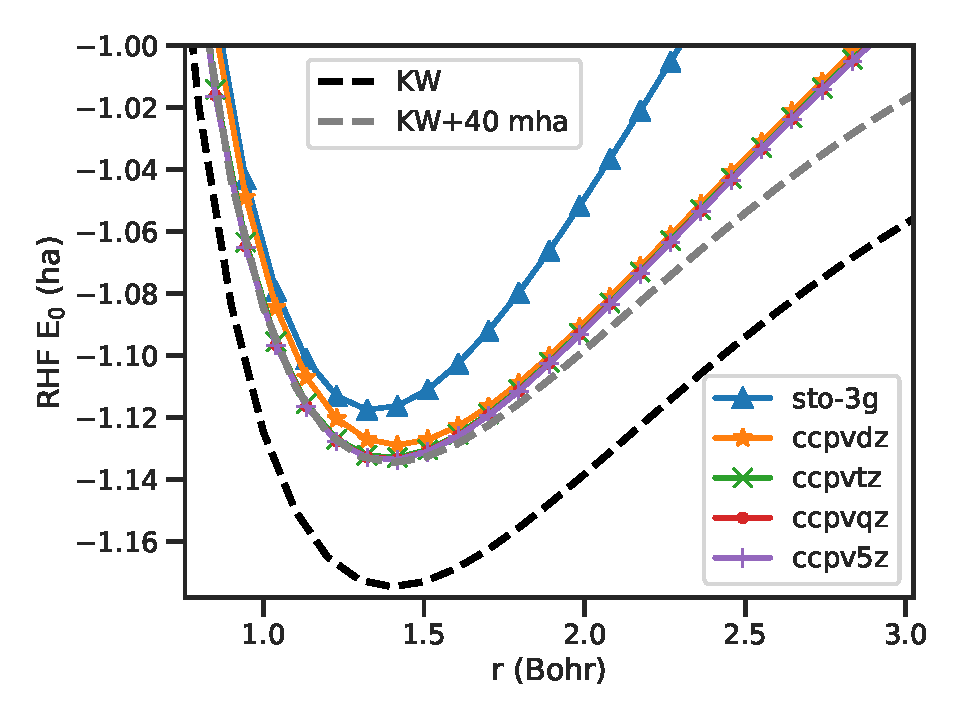
\includegraphics[width=0.6\linewidth]{f19a_h2-rhf-basis.pdf}
\caption{RHF electronic ground-state energy of H$_2$ in STO-3G and correlation consistent (cc) basis sets as compared to the exact values calculated by Kolos and Wolniewicz (KW)~\cite{Kolos1964}}
\label{fig:hf-h2}
\end{figure}

\subsubsection{Beyond Hartree-Fock}
Even when the complete basis set limit is reached, the HF solution is still not the exact electronic ground state due to its neglect of electron correlation.
One way to account for correlation effects is to perform a determinant expansion eq.~(\ref{eq:method-hf-ci}).
The unoccupied \emph{virtual} orbitals can be used to construct N-electron determinants that differ from the HF ground state by changing orbital occupation.
These determinants form a many-body basis, in which any wave function can be expressed as a linear combination.
This leads to the configuration interaction (CI) expansion, where the exact electronic ground state is expanded as a sum of determinants
\begin{align} \label{eq:method-hf-ci}
\psi_0 = \lim\limits_{M\rightarrow\infty}\sum\limits_{i=0}^{M} c_i \ket{D_i}.
\end{align}
If all determinants that differ by one particle-hole excitation from reference are considered, then we obtain a CI singles (CIS) expansion. If these and all determinants with two particle-hole excitations are considered, then the expansion is CI singles and doubles (CISD), etc.. If all excitations among a set of ``active'' orbitals are considered, then the expansion is said to involve the complete active space (CAS).

\subsubsection{Static and Dynamic Correlation}
The ground state is said to have \textit{static correlation} if one or more determinants in the exact expansion eq.~(\ref{eq:method-hf-ci}) are nearly degenerate with the reference determinant.
This will happen if there are virtual orbitals nearly degenerate with the highest occupied molecular orbital.
In contrast, the system has \textit{dynamic correlation} if the $c_i$ coefficients are small but non-zero for many determinants with high levels of excitation.
Dynamic correlation is often attributed to strong local correlation such as the electron-electron cusp condition.
The current definition of static and dynamic correlations is not precise~\cite{Benavides-Riveros2017}.
I introduce the above working definitions, because static correlation can be interpreted as a delocalization error due to fractional electron~\cite{Cohen2008}, and is related to the self-interaction error in density functional theory (DFT).
This bridges the languages used in quantum chemistry and condensed matter as well as points to a solution of the infamous ``bandgap problem'', to be introduced in  Sec.~\ref{sec:method-dft-bandgap}.

While the HF method enjoys much success in the study of atoms, its complete neglect of (Coulomb) electron correlation is woefully inadequate for many solids. The HF total energy is dominated by inner shell contributions, which overshadows the valence contributions important for correlated excitations in solids.
The HF energy eigenvalues show vanishing density of states at the Fermi level in metals and unphysically large band gaps in insulators~\cite{Perdew1981}.

\subsection{Kohn-Sham Density Functional Theory}

Using a mapping from electron density to total energy, density functional theory (DFT) is a method that can, in principle, exactly include electron correlation effects.
Though the exact density functional is unknown, even approximate functionals can lead to useful results.
DFT uses the three-dimensional total electron density $n(\bs{r})$ as the basic variable rather than the 3N-dimensional many-body wave function $\Psi(\bs{r}_1,\dots,\bs{r}_N)$. This is a dramatic simplification that likely lead to its dominance in modern electronic structure theory of solids and material science.

\subsubsection{The Hohenberg-Kohn theorems}
While having roots in Thomas-Fermi theory~\cite{Parr1989}, DFT was put on firm theoretical foundation by P. Hohenberg and W. Kohn (HK) in 1964~\cite{Hohenberg1964}, where they calculate the total electronic energy $E$ from an external potential $v(\bs{r})$ and a functional of the ground-state electron density
\begin{align}
E\equiv \int d\bs{r} n(\bs{r}) v(\bs{r}) + F[n(\bs{r})].
\end{align}
Two theorems are often attributed to this work:
\begin{definition}
\textit{V-representable density} A density $n(\bs{r})$ is V-representable if it is the ground-state density of some Hamiltonian $H$ in an external potential $v(\bs{r})$.
\end{definition}
\begin{theorem}
Assuming non-degenerate ground state, any V-representable ground-state density $n(\bs{r})$ uniquely determines its external potential $v(\bs{r})$. %(See extension to N-representable density by M. Levy)
\end{theorem}
\begin{proof}
by contradiction: Suppose there are two distinct external potentials $v$ and $v'$ that give rise to the same density $n$ via different hamiltonians $H$, $H'$ and wave functions $\Psi$ and $\Psi'$, respectively. By the variational principle $\braket{\Psi'|H'|\Psi'}+\braket{\Psi'|v'-v|\Psi'}=\boxed{\braket{\Psi'|H|\Psi'}>\braket{\Psi|H|\Psi}}=\braket{\Psi|H'|\Psi}+\braket{\Psi|v'-v|\Psi}>\braket{\Psi'|H'|\Psi'}+\braket{\Psi|v'-v|\Psi}$. Since $\Psi$ and $\Psi'$ give the same density, the local term $\braket{v'-v}$ cancels to give $\braket{\Psi'|H'|\Psi'}>\braket{\Psi'|H'|\Psi'}$, which is a contradiction.
\end{proof}
\begin{theorem}
Assuming number-conserving density variations that retain V-representability, the energy functional has a unique minimum at the ground-state density.
\end{theorem}
\begin{proof}
Consider an external potential $v$, its hamiltonian $H$, and its unique ground state $\Psi$ and density $n$. After a number-conserving variation, the new wave function $\Psi'$ can be used with the original hamiltonian and $\braket{\Psi'|H|\Psi'}>\braket{\Psi|H|\Psi}$ by the variational principle.
\end{proof}

These initial proofs by HK have two important assumptions: 1. the ground-state is non-degenerate and 2. the electron density $n(\bs{r})$ is V-representable. The latter is especially sever because reasonable densities were shown not to be V-representable~\cite{Levy1982,Lieb1983}. Fortunately, M. Levy proved that both assumptions can be weakened~\cite{Levy1979}. The HK theorems hold for N-representable densities regardless of ground-state degeneracy.
\begin{definition}
\textit{N representable density} A density $n(\bs{r})$ is N-representable if it can be obtained from some many-body wave function of N particles.
\end{definition}

While less publicized, HK also pointed out that the exact density functional less the direct/Column contribution can be calculated from a local energy-density functional $g_{\bs{r}}[n]$
\begin{align}
G[n]\equiv F[n]-\frac{1}{2}\int d\bs{r}d\bs{r}' \dfrac{n(\bs{r})n(\bs{r}')}{\vert\bs{r}-\bs{r}'\vert}=\int \bs{r} g_{\bs{r}}[n],\\
g_{\bs{r}}[n] \equiv \frac{1}{2}\nabla_{\bs{r}}\nabla_{\bs{r}'} n_1(\bs{r}, \bs{r}')\vert_{\bs{r}=\bs{r}'}+
\frac{1}{2}\int d\bs{r}' \dfrac{C_2(\bs{r}-\bs{r'}/2;\bs{r}+\bs{r}'/2)}{\vert\bs{r}'\vert},
\end{align}
which is constructed from one- and two-body reduced density matrices $n_1$ and $C_2$. They even went as far as to relate the leading-order behavior of the density functional to polarizability
\begin{align}
G[n] = G[n_0] + \int d\bs{r}d\bs{r}' K(\bs{r}-\bs{r}')\tilde{n}(\bs{r})\tilde{n}(\bs{r}')+h.o.,
\end{align}
where $\tilde{n}$ is a small number-conserving density variation and the kernel $K$ is related to the polarizability in reciprocal space
\begin{align}
K(\bs{r}-\bs{r}') = \dfrac{1}{\Omega}\sum\limits_{\bs{q}} K(\bs{q}) e^{-i\bs{q}\cdot(\bs{r}-\bs{r}')}, \\
K(\bs{q}) = \dfrac{2\pi}{q^2}\left[ \frac{1}{\alpha(\bs{q})}-1 \right] = \dfrac{2\pi}{q^2}\dfrac{1}{\epsilon(\bs{q})},
\end{align}
where $\alpha(\bs{q})$ and $\epsilon(\bs{q})$ are the polarizability and dielectric constant, respectively. The HK theorems and limits provide some checks for practical parametrization of the exact density functional. Unfortunately, they provide no guidance on how one might start to construct numerical approximations to the exact functional.

\subsubsection{The Kohn-Sham equations}

One year after HK, W. Kohn and L. J. Sham (KS)~\cite{Kohn1965} worked out practical guidelines for constructing approximations to the exact density functional. KS first partitioned the total energy to highlight the least-understood ``exchange-correlation" term $E_{xc}[n]$.
\begin{align} \label{eq:ks-etot}
E=\int d\bs{r} n(\bs{r}) v(\bs{r}) + \frac{1}{2}\int d\bs{r}d\bs{r}' \dfrac{n(\bs{r})n(\bs{r}')}{\vert\bs{r}-\bs{r}'\vert} + T[n] + E_{\text{xc}}[n],
\end{align}
where $T$ is a kinetic energy functional. KS then approximated $E_{xc}$ by the corresponding contribution in the homogeneous electron gas, the local density approximation (LDA)
\begin{align}
E_{\text{xc}}[n] = \int d\bs{r}n(\bs{r})\epsilon_{\text{xc}}(n(\bs{r})).
\end{align}
Next, by minimizing eq.~(\ref{eq:ks-etot}) with respect to number-conserving density variation, they obtained the stationary condition for the ground-state density
\begin{align}
\int \delta n \left[
\dfrac{\delta T[n]}{\delta n}+
v(\bs{r}) + \int d\bs{r}' \dfrac{n(\bs{r}')}{\vert\bs{r}-\bs{r}'\vert}+
\dfrac{d(n\epsilon_{\text{xc}}(n))}{dn}
\right] = 0. \label{eq:ks-dn}
\end{align}
To solve eq.~(\ref{eq:ks-dn}), KS \textit{assumed} that the ground-state density $n$ came from an auxiliary system of non-interacting electrons, i.e., a Slater determinant. This KS \textit{ansatz} turns eq.~(\ref{eq:ks-dn}) into a system of one-particle equations of non-interacting particles in some effective potential $v^{\text{eff}}_{KS}$ determined by the density $n(\bs{r})$. Most practical implementations of DFT use the KS auxiliary-system formulation.

Practical success of the DFT LDA method was not realized until 1981, when J. P. Perdew and A. Zunger (PZ)~\cite{Perdew1981} parametrized exact quantum Monte Carlo data of the homogeneous electron gas, obtained by D. M. Ceperley and B. J. Alder~\cite{Ceperley1980} the year prior. PZ's eq.~(13-17) define the KS-DFT method and the LDA we use today. The electron density for spin $\sigma$ is a sum of occupied spin orbitals squared
\begin{align}
n_{\sigma} = \sum\limits_{\sigma}\sum\limits_{a=1}^{N_{\sigma}}
f_{a\sigma} \vert\psi_{a\sigma}(\bs{r})\vert^2,
\end{align}
where the occupation numbers $f_{a\sigma}\in[0, 1]$, and the kinetic energy is the sum of contributions from all occupied spin orbitals of the non-interacting system
\begin{align}
T_s[n] = \sum\limits_\sigma\sum\limits_{a=1}^{N_{\sigma}}
f_{a\sigma} \braket{\psi_{a\sigma}|-\frac{1}{2}\nabla^2|\psi_{a\sigma}}.
\end{align}
Minimizing eq.~(\ref{eq:ks-etot}) with the constraint that the spin orbitals remain orthonormal, PZ obtains
\begin{align}
\dfrac{\delta}{\delta\psi_{a\sigma}} \left[
T_s[n] + \int d\bs{r}v(\bs{r}) + \int d\bs{r}\int d\bs{r}' \dfrac{n(\bs{r}')}{\vert\bs{r}-\bs{r}'\vert} +
\dfrac{\delta}{\delta n_{\sigma}} E_{xc}(n_{\up},n_{\dn})
\right].
\end{align}

\subsubsection{The Band Gap Problem} \label{sec:method-dft-bandgap}
The Kohn-Sham eigenvalues do not have the same physical meaning as the Hartree-Fock eigenvalues as given by Koopmans theorem. Thus, a band gap ``problem'' arises when one compares the HOMO-LUMO gap from KS-DFT to experimental measurements of the fundamental gap $E_g$. The eigenvalue of the Kohn-Sham HOMO can be identified with the ionization energy of an isolated molecule if the exchange-correlation potential vanish at infinity.
This is a special case, because the ionization energy is dominated by the long-range asymptotic behavior of the 1RDM, which is determined by the long-range tail of the electronic density with no contribution from the short-sighted exchange correlation potential.

When extended to handle systems with fractional electron number, the derivative discontinuity of the exact density functional is $E_g$. It has contribution from both the non-interacting kinetic functional $T_s[n]$ and the exact exchange-correlation functional $E_{xc}[n]$. The KS HOMO-LUMO gap measures the derivative discontinuity in $T_s[n]$. However, as shown in Fig.~\ref{fig:method-dft-smooth-lda}, the $E_{xc}[n]$ under LDA is smooth, so its contribution to the gap is missing. As a result, the LDA gap is $\sim 50\%$ that of experiment, showing that the derivative discontinuity in $E_{xc}[n]$ can be of similar magnitude as the gap and cannot be ignored.

\begin{figure}[h]
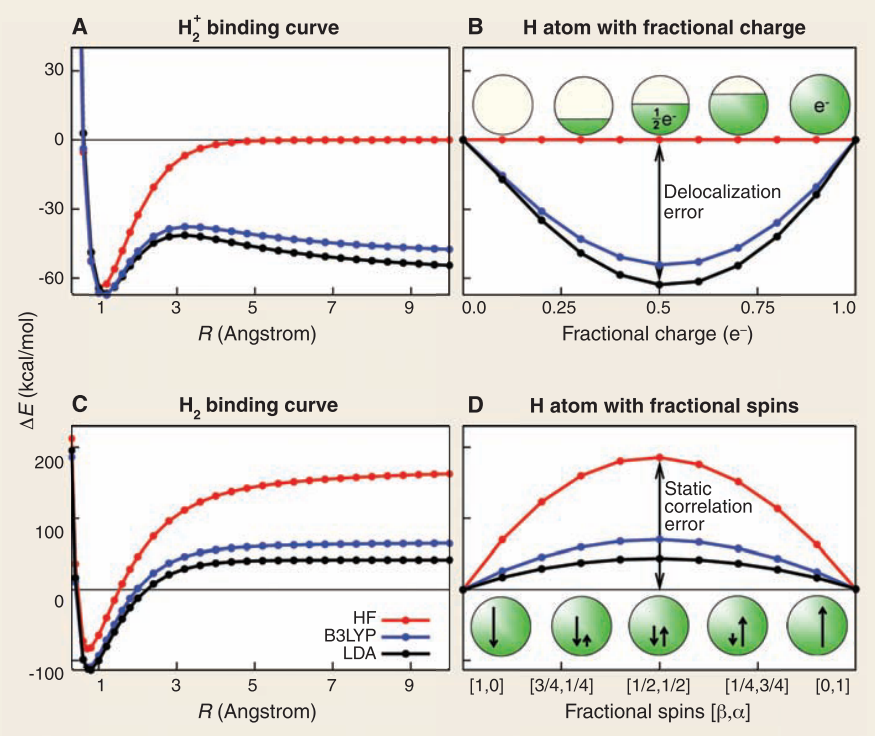
\includegraphics[width=0.45\linewidth]{cohen2008-fig1.png}
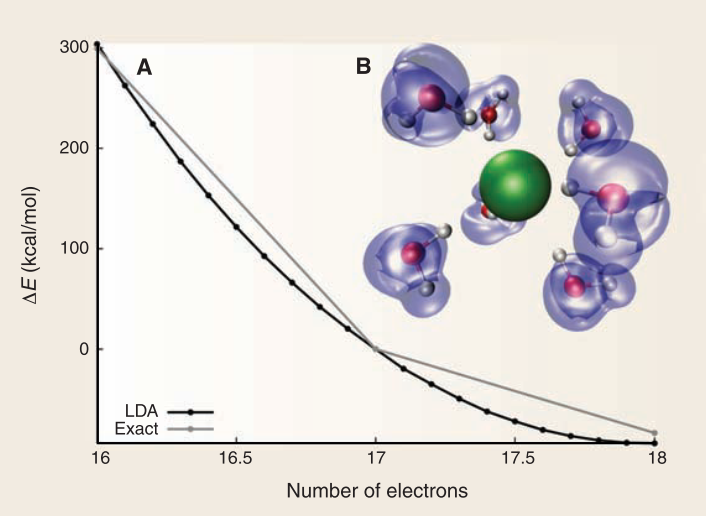
\includegraphics[width=0.52\linewidth]{cohen2008-fig2.png}
\caption{A. J. Cohen, P. Mori-S\'anchez, and W. Yang~\cite{Cohen2008} explains that the self-interaction error in H$_2^+$ binding curve (left panel A) is due to the presence of fractional electron (left panel B), which leads to a delocalization error when LDA is used.}
\label{fig:method-dft-smooth-lda}
\end{figure}

% Q/ why is HSE so good?
% A/ because it has both convex and concave components. See Cohen 2008 Fig. 2

\subsubsection{Beyond Local Density Approximation}

While extremely successful, the LDA has well-documented deficiencies.
As discussed in Sec.~\ref{sec:method-dft-bandgap}, LDA underestimates the band gap due to a lack of derivative discontinuity.
Further, it tends to overestimate the binding energy of molecular systems. This is attributed to the logarithmic divergence of the LDA correlation functional as density tends to infinity (see eq.~(7.55) in Ref.~\cite{Giuliani2005}).
%For an isolated atom, the LDA xc potential approaches zero exponentially fast at large distances rather than the correct asymptotic limit $-e^2/r$.

The logarithmic divergence of the LDA is largely corrected by the generalized gradient approximation (GGA). This modification is not as straight-forward as adding an extra term that depends on the gradient of the electron density $\bs{\nabla}n$ to the exchange-correlation function. An arbitrary choice of the gradient term can distort the xc hole and break the sum rule that controls its global strength
\begin{align}
\int\bs{r}' n(\bs{r}')[g(\bs{r},\bs{r}')-1] = -1.
\end{align}
J. Perdew and co-workers overcame this difficulty by introducing a real-space cutoff to the exchange hole. While the details are technical, the final form of the GGA exchange functional is elegant
\begin{align} \label{eq:method-dft-pbe-x}
E_x^{GGA}[n] = \int d\bs{r} n(\bs{r})\epsilon_x(n(\bs{r}))F_x(\bs{s}(\bs{r})),
\end{align}
where $\epsilon_x$ is the LDA exchange function and the scaled gradient
\begin{align}
\bs{s}(\bs{r}) = \dfrac{\bs{\nabla}n(\bs{r})}{2k_F(\bs{r})n(\bs{r})}.
\end{align}
A simple form for the \emph{exchange enhancement factor} $F_x$ was given by J. Perdew, K. Burke, and E. Ernzerhof~\cite{Perdew1996} in 1996. After another careful cutoff on the correlation functional, the immensely popular PBE functional was constructed. The PBE xc functional takes the same form as eq.~(\ref{eq:method-dft-pbe-x}), but with a different enhancement factor: $F_{xc}$ instead of $F_x$.
PBE softens molecular bonds relative to the LDA and predicts an order of magnitude more accurate dissociation energies of many molecules~\cite{Perdew1996}.

Unfortunately, both LDA and PBE suffer from a well-known failure of any local and semi-local density functional theory: the absence of Van der Waals interaction.
This interaction is entirely due to the correlation of density fluctuations and is dominant for two neutral objects with non-overlapping electron densities.
When fluctuation creates an instantaneous dipole moment in one electron distribution, it induces an anti-aligned dipole moment in the other.
The van der Waals interaction is thus attractive and decays as dipole-dipole interaction strength, $\frac{1}{r^6}$, in the separation distance $r$ between the centers of the two distributions.
While KS-DFT relies on the average electron density of a non-interacting system, it is still possible to include the contribution of Van der Waals interaction in the density functional.
Consider the Coulomb interaction as a perturbation to two widely separated atoms, one can show that the interaction energy is proportional to a convolution of the density-density response functions of the isolated atoms
\begin{align}
\braket{\hat{H}_{12}} = -\dfrac{\hbar}{2\pi}
\int d\bs{r}_1d\bs{r}_1'
\int d\bs{r}_2d\bs{r}_2'
\dfrac{e^2}{\vert\bs{r}_1-\bs{r}_2\vert}
\dfrac{e^2}{\vert\bs{r}_1'-\bs{r}_2'\vert} \nonumber \\
\times\int\lim\limits_0^{\infty}
\chi_1(\bs{r}_1, \bs{r}_1')
\chi_2(\bs{r}_2, \bs{r}_2') + h.o.,
\end{align}
as written in eq.~(7.116) in Ref.~\cite{Giuliani2005}. One can then proceed to approximate the density-density response function using the static electron density, e.g. using the polarizability of the homogeneous electron gas.

Finally, exact-exchange functionals such as PBE0 and HSE~\cite{Heyd2003} have been developed for atoms having localized valence electrons, e.g., with d or f angular momentum.
These functionals are crucial in the study of magnetism, as the PBE functional overly favor delocalized electrons and often predict qualitatively wrong magnetic momentum and spin orderings of transition metals.
However, these exact-exchange functionals were never a focus throughout this thesis, so I will not go into details here.
%exact exchange functionals (HSE)
%SCAN?
